\section{Introduction}

Time series forecasting is a cornerstone of decision-making in critical domains such as energy, healthcare, and supply chains~\cite{rezaei2021stock,tzelepi2023deep,sun2022accurate,idrees2019prediction,kiyasseh2021clocs,liu2025towards,lei2026hierarchical}. Recently, the field has witnessed a paradigm shift from training task-specific models from scratch~\cite{zhou2021informer,wu2021autoformer,zhou2022fedformer,wu2023timesnet,liu2023itransformer,lyu2025occamvts} to \textit{Time Series Foundation Models} (TSFMs)~\cite{das2024decoder,goswami2024moment,liu2024timer,liu2025sundial,xiao2025timefound,graf2025flowstate}, which are pre-trained on diverse corpora to learn transferable temporal representations. However, a critical gap~\cite{hinder2024one,wen2023onenet,zhao2025proactive,jin2022domain,he2023domain,zhonglearning,zhong2026learning} remains between pre-training and deployment: real-world domain shifts (e.g., scale changes, seasonal discrepancies, sensor variations) can severely degrade the performance of frozen TSFMs.

To bridge this gap, existing adaptation strategies primarily fall into two paradigms (As shown in \autoref{fig:paradigm}):

% However, a significant gap ~\cite{hinder2024one,wen2023onenet,zhao2025proactive,jin2022domain,he2023domain,zhonglearning,zhong2026learning} remains between pre-training and deployment: in real-world forecasting, domain shifts often manifest as level/scale changes, seasonal-pattern discrepancies, sensor calibration differences, and sampling-rate mismatches. These shifts can substantially degrade the performance of frozen TSFMs in long-horizon forecasting. To bridge this gap for TSFM-based forecasting, existing adaptation strategies primarily fall into two paradigms:


% real-world data often exhibit severe distribution shifts and domain heterogeneity, necessitating effective adaptation to target domains~\cite{hinder2024one,jin2022domain,he2023domain}. To address this, current adaptation strategies primarily fall into two paradigms:

% os with limited task-specific engineering~\cite{ekambaram2024tiny,shi2024time,liu2024moirai,ansari2024chronos,woo2024unified,ansari2025chronos}. 

\begin{figure}[t]
  \centering
  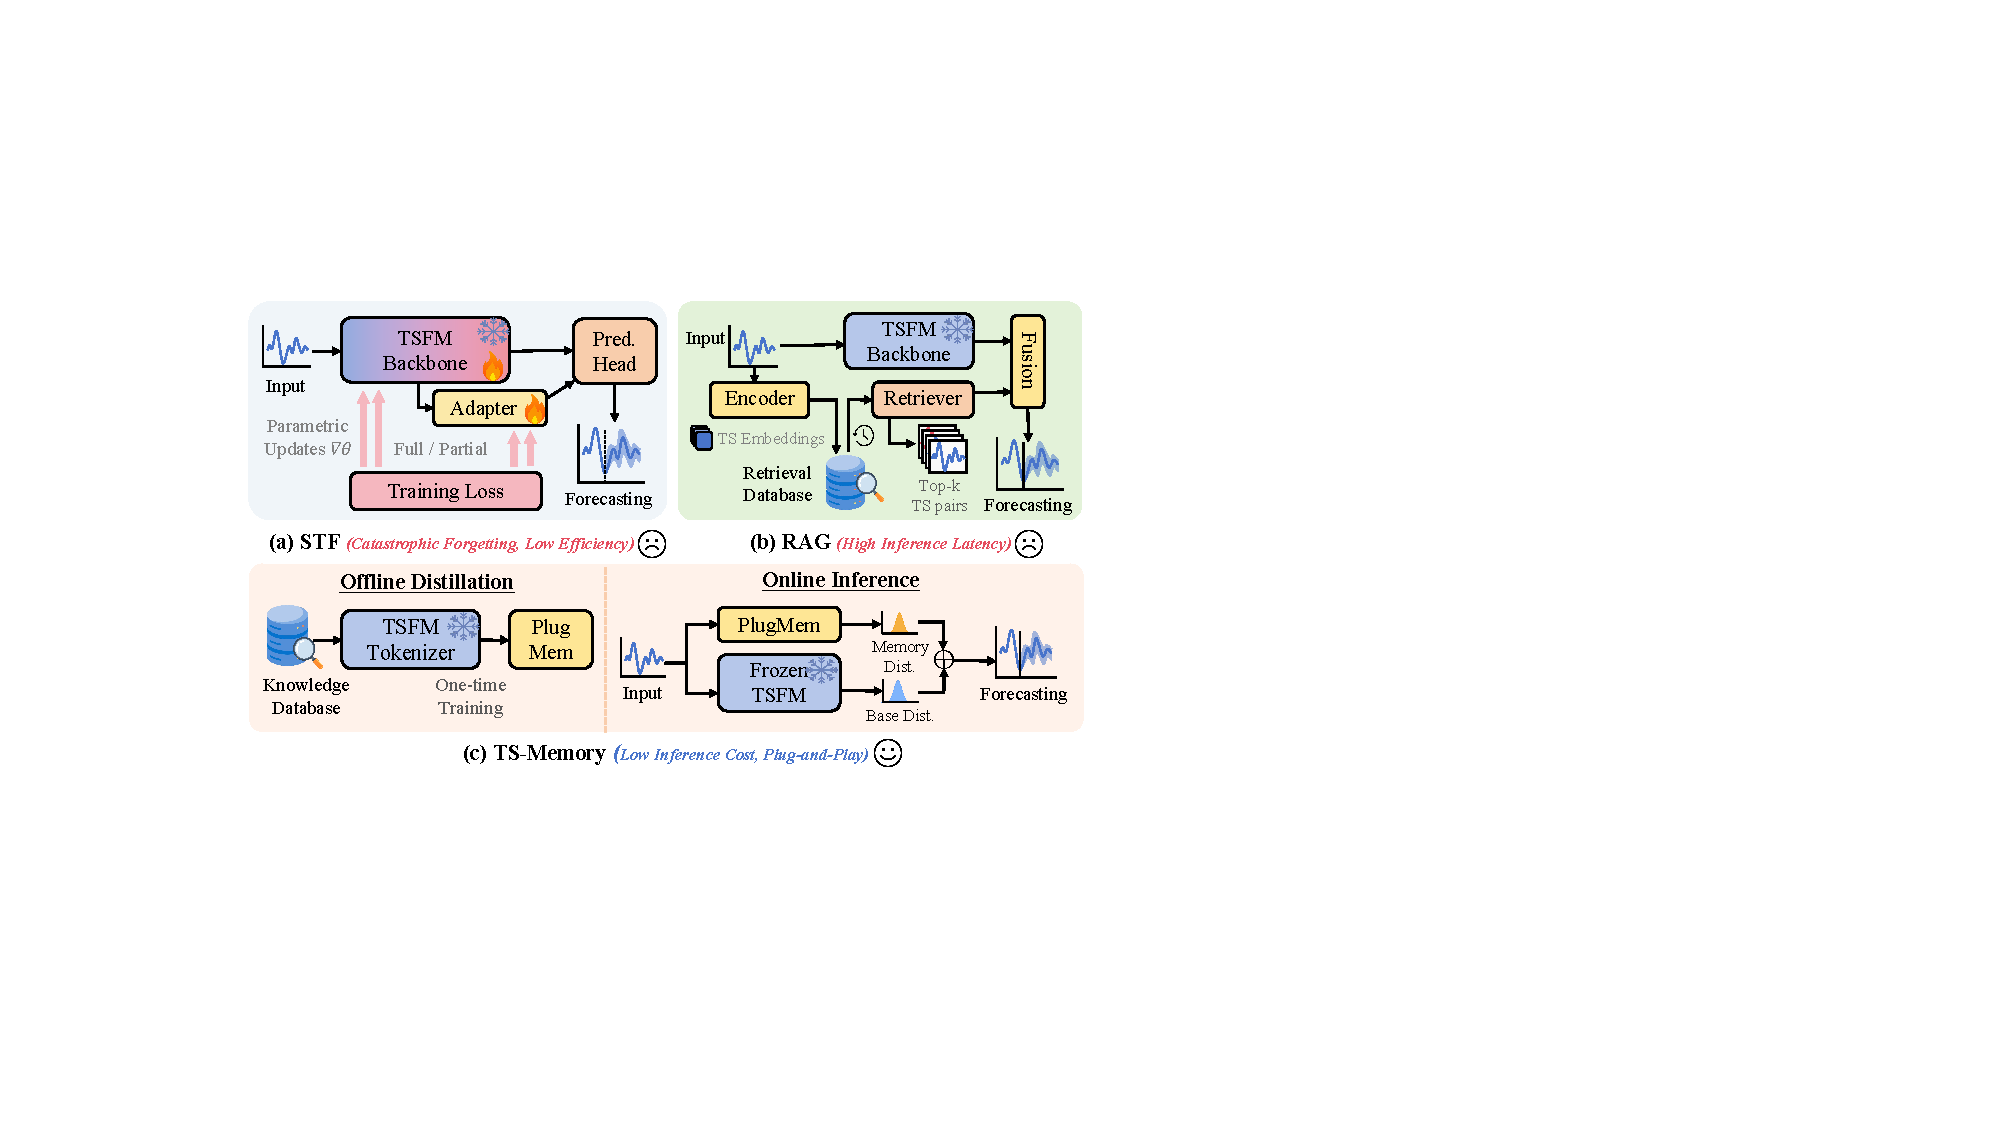
\includegraphics[width=\linewidth]{figures/paradigm.pdf}
  % \caption{Comparison of TSFM adaptation paradigms: \textbf{(a)} Parametric Adaptation updates backbone weights, risking catastrophic forgetting and high maintenance costs; \textbf{(b)} Non-Parametric Retrieval relies on costly inference-time external database searches; \textbf{(c)} Parametric Memory Distillation (ours) distills retrieval knowledge into a lightweight plug-and-play module for efficient frozen-backbone adaptation.}

    \caption{Comparison of TSFM adaptation paradigms: \textbf{(a)} Parametric Adaptation; \textbf{(b)} Non-Parametric Retrieval; \textbf{(c)} Parametric Memory Distillation (Ours).}
  
  \Description{Comparison of TSFM adaptation paradigms}
  \label{fig:paradigm}

\end{figure}


% \begin{enumerate}[leftmargin=*]
%     \item \textbf{Parametric Adaptation:} Methods such as full or parameter-efficient fine-tuning adapt model weights to the target domain~\cite{gupta2024low,gupta2024beyond,qiao2025multi,zhao2025less}. While effective, this approach necessitates maintaining a separate model copy for every domain, incurring prohibitive storage and maintenance costs. Furthermore, continuous updates on frozen backbones risk catastrophic forgetting ~\cite{fu2025financial,beichter2025decision,yu2025time} of general knowledge acquired during pretraining~\cite{ning2025mode,lee2025lightweight,sheng2023s,ye2023mlora,karaouli2025time,luo2025empirical}.

%     \item \textbf{Non-Parametric Retrieval:} To preserve the frozen backbone, methods like Metric Matching~\cite{vinyals2016matching,snell2017prototypical,sung2018learning} or Retrieval-Augmented Generation (RAG) retrieve historical instances from an external database at inference time~\cite{lewis2020retrieval,jing2022retrieval,liu2024retrieval,yang2025timerag,han2025retrieval,ning2025ts}. While this avoids weight updates, it places heavy index maintenance and kNN queries on the \textit{critical inference path}. The latency and computational cost scale linearly with the size of the external knowledge base, making such methods prohibitive for real-time or edge deployment~\cite{fan2024survey,ning2025ts,jin2025ragcache,zhu2024accelerating,asai2024reliable}.
% \end{enumerate}

\begin{enumerate}[leftmargin=*]
    \item \textbf{Parametric Adaptation:} Methods like full or parameter efficient fine-tuning adapt model weights to the target domain~\cite{qiao2025multi,zhao2025less,ruan2025st}. Despite their effectiveness, this approach requires maintaining a distinct model copy for each domain, leading to exorbitant storage and maintenance costs. Moreover, continuous updates to frozen backbones risk catastrophic forgetting~\cite{fu2025financial,beichter2025decision,yu2025time} of general pre-training knowledge~\cite{ning2025mode,lee2025lightweight,ye2023mlora,karaouli2025time}.

    \item \textbf{Non-Parametric Retrieval:} To preserve the frozen backbone, methods like Metric Matching~\cite{vinyals2016matching,snell2017prototypical,sung2018learning} and Retrieval Augmented Generation (RAG) retrieve historical instances from an external database during inference~\cite{lewis2020retrieval,jing2022retrieval,liu2024retrieval,yang2025timerag,han2025retrieval,ruan2025rastretrievalaugmentedspatiotemporal}. While this avoids weight updates, it places heavy index maintenance and kNN queries on the \textit{critical inference path}. The latency scales linearly with the size of the external knowledge base, making such methods prohibitive for real-time or edge deployment~\cite{fan2024survey,ning2025ts,jin2025ragcache,zhu2024accelerating,asai2024reliable,lei2025game} under tight latency constraints.
\end{enumerate}


% \textbf{2) Search-based retrieval}: This paradigm augments frozen models by retrieving similar historical instances from an external database at inference. A lightweight variant is metric-based matching, which represents the target domain with a small support set and predicts by matching query contexts to support embeddings or prototypes following classic metric-based few-shot learning~\cite{vinyals2016matching,snell2017prototypical,sung2018learning}. A more powerful yet computationally heavier variant is Retrieval Augmented Generation (RAG), which retrieves relevant historical time series segments and their future trajectories from a large knowledge base, conditioning forecasting on these exemplars to enhance robustness~\cite{lewis2020retrieval,jing2022retrieval,liu2024retrieval,yang2025timerag,han2025retrieval,ning2025ts}.

% Existing methods face a dilemma between \textit{maintenance} efficiency (model adaptation per domain) and \textit{inference} efficiency (runtime search cost). This raises a question: \textit{Can we capture the adaptability of retrieval-based methods without their inference-time latency?}

Existing methods face a dilemma between \textbf{maintenance} (per-domain model adaptation) and \textbf{inference} efficiency (runtime search cost). This raises a key question: \textit{Can we capture the robust adaptability of retrieval-based methods while maintaining the constant-time inference and deployment simplicity of parametric adapters?}

%\vspace{0.3em}
% In this paper, we propose a third paradigm: \textbf{Parametric Memory Distillation}. Our key insight is that the "knowledge" provided by online retrieval—specifically, the distribution of future predictions implied by similar historical inputs—can be \textit{distilled} from a non-parametric database into a compact, parametric module. By shifting the \emph{heavy} lifting of search to an offline training stage, we replace the external database with a \emph{lightweight} neural memory. 

% We answer this with a third paradigm: \textbf{Parametric Memory Distillation}. Our core idea is to distill retrieval-based knowledge into a compact parametric module, where this knowledge captures the distribution of future predictions conditioned on similar historical patterns. By performing retrieval offline during training, we eliminate the need for external databases at inference time and replace them with a lightweight neural memory. 

% As show in figure 1,In this work, we distill the predictive distribution induced by retrieval, rather than storing or querying retrieved instances at test time. Concretely, retrieval provides distributional corrections to the frozen TSFM’s base forecast, and we distill these corrections into a small parametric memory module. 

We propose a third paradigm: \textbf{Parametric Memory Distillation} (Table~\ref{tab:match_rag_tsmemory}). Our core insight is that the "knowledge" provided by online retrieval, namely the predictive distribution implied by similar inputs, can be compiled offline into a compact neural module. By shifting retrieval cost to training, we decouple retrieval benefits from runtime costs. Concretely, we introduce \textbf{TS-Memory}, a plug-and-play adapter for frozen TSFMs. Unlike RAG, which queries a datastore at every inference step, TS-Memory learns to approximate the teacher distribution from an offline kNN retriever. During inference, it serves as an internalized memory of domain patterns that fuses seamlessly with the TSFM's predictions.

% We answer this with a third paradigm: \textbf{Parametric Memory Distillation} (Table~\ref{tab:match_rag_tsmemory}). Our core insight is that the "knowledge" provided by online retrieval, namely the distribution of future predictions implied by similar historical inputs, can be \textit{compiled} offline into a compact neural module. By shifting the search computational burden to the training stage, we decouple retrieval benefits from runtime costs. Building on this, we introduce \textbf{TS-Memory}, a plug-and-play adapter for frozen TSFMs. Unlike RAG (which queries a database at runtime), TS-Memory learns to approximate the \textit{teacher distribution} from an offline kNN retriever. During inference, TS-Memory acts as a fast, distinct "memory" of domain patterns that fuses seamlessly with the TSFM's predictions. 

% \item We address this with a third paradigm: \textbf{Parametric Memory Distillation} (Table~\ref{tab:match_rag_tsmemory}). Our core insight is that the "knowledge" from online retrieval—specifically, the future prediction distribution implied by similar historical inputs—can be \textit{compiled} offline into a compact neural module. By shifting the search computational burden to the training stage, we decouple retrieval benefits from runtime costs. Building on this, we introduce \textbf{TS-Memory}, a plug-and-play adapter for frozen TSFMs. Unlike RAG (which queries a database at runtime), TS-Memory learns to approximate the \textit{teacher distribution} from an offline kNN retriever. During inference, TS-Memory serves as a fast, dedicated "memory" of domain patterns that fuses seamlessly with TSFM predictions.


This approach satisfies three critical deployment requirements: (1) \textbf{Zero Inference Search:} It eliminates dependencies on external vector databases during runtime; (2) \textbf{Constant Time Complexity:} Inference latency is $O(1)$, independent of the historical data size; (3) \textbf{Non-Destructive Adaptation:} It bypasses the risk of catastrophic forgetting by keeping the backbone frozen. As visualized in Figure~\ref{fig:paradigm}, TS-Memory bridges the gap between parametric adaptation and non-parametric retrieval. Rather than storing or querying retrieved instances at test time, we distill the \emph{distributional corrections} that retrieval induces on the frozen TSFM's base forecast into a lightweight neural memory module. This preserves the frozen backbone to prevent forgetting, adapts to local domains as RAG does, and operates with the speed of a standard forward pass.

% Specifically, as shown in Figure~\ref{fig:paradigm}, we distill the predictive distribution induced by retrieval rather than storing or querying retrieved instances at test time. Retrieval provides distributional corrections to the frozen TSFM's base forecast, and we compress these corrections into a lightweight neural memory module.


% Our key insight is that the "knowledge" provided by online retrieval—specifically, the distribution of future predictions implied by similar historical inputs—can be \textit{distilled} from a non-parametric database into a compact, parametric module. By shifting the \emph{heavy} lifting of search to an offline training stage, we replace the external database with a \emph{lightweight} neural memory.


%\vspace{0.3em}
% Building on this idea, we introduce \textbf{TS-Memory}, a plug-and-play memory module designed for frozen TSFMs. Unlike RAG, which queries a database during runtime, TS-Memory learns to approximate the \textit{teacher distribution} induced by an offline kNN retriever. During inference, TS-Memory acts as a fast, distinct "memory" of domain patterns that fuses seamlessly with the TSFM's predictions.

%\vspace{0.3em}
% This approach satisfies three critical deployment requirements: (1) \textbf{Offline Compilation:} No dependence on runtime retrieval engines or external indices; (2) \textbf{Constant Overhead:} Inference latency is low and independent of the knowledge base size; (3) \textbf{Universal Compatibility:} The module connects to frozen backbones without architectural modification. As visualized in Figure~\ref{fig:paradigm}, TS-Memory bridges the gap between parametric adaptation, which updates backbone weights at the cost of catastrophic forgetting and high maintenance, and non-parametric retrieval, which relies on costly inference-time external database searches. By distilling retrieval knowledge into a lightweight plug-and-play module, TS-Memory fully retains the frozen backbone (preventing forgetting) and adapts to local domains (like RAG), yet still operates with the speed of a standard neural network.


%\vspace{0.3em}

Technically, TS-Memory operates in two phases. First, during an offline stage, we construct a \textit{privileged supervision} by retrieving $k$-nearest neighbors for training instances and aggregating their future trajectories into \emph{quantile targets}. This process captures the non-parametric uncertainty inherent in the data. Second, we train a lightweight parametric memory module to predict these teacher quantiles directly from the input context. To ensure robustness, we employ a \textit{confidence-gated memory distillation} that selectively transfers knowledge only when retrieval provides reliable signals. During inference, the memory module functions as a plug-and-play addition to the frozen TSFM, fused via linear interpolation to enhance adaptability without incurring any search latency.

%\vspace{0.3em}
Our contributions are summarized as follows:
\begin{itemize}[leftmargin=*]
    \item \textbf{Paradigm Shift:} We propose the Parametric Memory Distillation framework for TSFMs, transforming expensive online retrieval into a learnable, offline memory mechanism.
    
    \item \textbf{TS-Memory:} We design a lightweight module that distills non-parametric kNN distributions into parametric representations, featuring a novel distribution fusion interface for frozen TSFMs.
    
    \item \textbf{Efficiency \& Performance:} Extensive experiments demonstrate that TS-Memory outperforms representative methods from both paradigms in accuracy while significantly reducing inference latency, offering a superior trade-off for practical deployment.
\end{itemize}


% \begin{table}[b]
%   \centering
%   \vspace{-1em}
%   \caption{Comparison of metric-based matching, RAG for TS, and Memory for TS.}
%   \label{tab:match_rag_tsmemory}
%   \vspace{-1em}
% \footnotesize
%   \setlength{\tabcolsep}{2pt}
%   \renewcommand{\arraystretch}{1.1}
%   \scalebox{0.95}{
%   \begin{tabular}{lcccc}
%     \toprule
%     Method & Inference search? & External state & Overhead scaling & How to adapt \\
%     \midrule
%     Metric match & Yes ($|S|$) & Support/Proto & $O(|S|)$ & Swap $S$ \\
%     RAG for TS & Yes ($|K|$) & Knowledge Base & $O(|K|)$ & Swap KB \\
%     Memory for TS & No & Mem Params & $O(1)$ & Train Mem \\
%     \bottomrule
%   \end{tabular}
%   }

% \end{table}



\begin{table}[t]
  \centering

  \caption{Comparison of TSFM adaptation paradigms. TS-Memory combines low latency with low storage cost.}
  \label{tab:match_rag_tsmemory}

  \footnotesize
  \setlength{\tabcolsep}{3pt}
  \renewcommand{\arraystretch}{1.2}
  \scalebox{0.86}{
  \begin{tabular}{lcccccc}
    \toprule
    Paradigm & Inference & Deployment & Latency & Backbone & Plug and\\
    & Search? & Cost & Scaling & Status &Play?\\
    \midrule
    Parametric Adaptation & No & High (Model Copies) & $O(1)$ & Updated & No\\
    Non-Parametric Retrieval & Yes & High (Vector DB) & $O(|\mathcal{D}|)$ & Frozen & Yes\\
    \rowcolor{gray!10} \textbf{Parametric Distillation} & \textbf{No} & \textbf{Low (Tiny Module)} & $\mathbf{O(1)}$ & \textbf{Frozen} & \textbf{Yes}\\
    \bottomrule
  \end{tabular}
  }

\end{table}